\documentclass[10pt,a4paper,oneside]{article}
\usepackage[utf8]{inputenc}
\usepackage[english]{babel}
\usepackage{amsmath}
\usepackage{amsfonts}
\usepackage{amssymb}
\usepackage{graphicx}
%personal preferences for hyperlinks 
\usepackage[hidelinks]{hyperref}
\hypersetup{colorlinks=true}
%changing the separator before a figure's caption
\usepackage[labelsep=space]{caption}
\usepackage{listings}

\usepackage{url}
%added to allow for spaces to be added to paths and url's
\makeatletter
\begingroup \lccode`+=32 \lowercase
 {\endgroup \def\Url@ObeySp{\Url@Edit\Url@String{ }{+}}}
 \def\Url@space{\penalty\Url@sppen\ }
\makeatother

%change font
\usepackage[T1]{fontenc}
\renewcommand{\familydefault}{\sfdefault} %computer modern sans serif

%changing the margins 
\usepackage[left=2.5cm, top=2.5cm,right=2.5cm, bottom=2.5cm]{geometry}
 \tolerance=100000  % all 3 of these commands make LaTeX less fussy about what
\hbadness=10000  % is a "good'' length/width/height of a page
\raggedbottom

%I did not find a reason why Latex was creating a blank page at the begining 
%this fixes it
\usepackage{atbegshi}% http://ctan.org/pkg/atbegshi
\AtBeginDocument{\AtBeginShipoutNext{\AtBeginShipoutDiscard}}

%document title, no date 	
\title{Linux installation guide for Abaqus 2017}
\date{}

\begin{document}
\textbf{\maketitle}
\section{Licensing notes}
Before installing Abaqus make sure you have read and understood the license requirements, in particular noting:
\begin{itemize}
\item Only appropriate authorised support staff may make physical copies of the software or documentation. 
\item Abaqus might only be installed on computers owned by the University of Sheffield, it might not be installed on computers owned by staff or students
\end{itemize}

\section{Supported Linux versions}
The following distributions are fully supported:
\begin{itemize}
\item Red Hat Enterprise Linux Server
	\subitem Red Hat Enterprise Linux Server 6.x, where x=>5, is a Compatible platform
	\subitem Red Hat Enterprise Linux Server 7.1 is a Qualified platform
	\subitem Red Hat Enterprise Linux Server 7.x, where x=0 or x>1, is a Compatible platform
\item SuSE Linux Enterprise Server
	\subitem SuSE Linux Enterprise Server 11 SP3 is a Validated platform
	\subitem SuSE Linux Enterprise Server 11 SPx, where x>3, is a Compatible platform
	\subitem SuSE Linux Enterprise Server 12 SP1 is a Validated Platform
	\subitem SuSE Linux Enterprise Server 12 SPx, where x=0 or x>1, is a Compatible platform

\end{itemize}

\section{Supported compilers for Abaqus 2017}
Some Abaqus functionality (e.g. UMAT subroutines) requires Fortran and C++ compilers. Therefore before installing Abaqus install the following two compilers:
\begin{itemize}
\item Fortran compiler:Intel Fortran Compiler XE 2016 Update 1 (available at the University of  Sheffield \href{https://cics.dept.shef.ac.uk/software/}{Software donwload service}.

\item C++ compiler: GCC. Enter the following line in a terminal window:
\begin{lstlisting}[language=bash]
yum install gcc -c++
\end{lstlisting}

\end{itemize}

\textbf{Note}: do not install \textbf{Tosca Fluid} unless you have one of the  required fluid dynamics solvers \textbf{Fluent} or \textbf{Star-CCM} installed on your computer, otherwise the installation will fail.
\\
Note the installation will require around 11Gb temporarily for a complete install of the products and documentation. You will also need to have the openmotif and $compat-libstdc++-33$ packages installed on Red Hat systems.


\section{Installation}
\begin{enumerate}
\item Download the .iso image following the instructions provided in the email from the software download service.
\item Mount the .iso file e.g. as \textbf{root} enter 
\begin{lstlisting} 
mount -o loop 'Abaqus2017.iso' /mnt/disk 
\end{lstlisting}
\item The above command will mount the image at \textbf{/mnt/disk}, assuming this is the location you chose. To start the suit installer run the following script <location>/Abaqus2017/1/StartGUI.sh

There are 4 installers which need to be run in the following order:
\begin{enumerate}
\item Abaqus documentation (optional)
\item Abaqus Services (solvers)
\item CAA developer software
\item Abaqus/CAE (interactive GUI)
\end{enumerate}

\textbf{Important:} you must always install both the Abaqus services (solvers) and Abaqus/CAE. They cannot be installed separately or individually.

When you start the installer, you can choose which product or products to install. Once you have made this selection, individual installers will run for each product. Most defaults values are given and it is recommended that you accept those values. Required changes will be specified in this guide. \bigskip

Once the Installer has started select the components you want to install and click Next (Fig. \ref{fig:abaqus1}).
\begin{figure}[h]
\centering
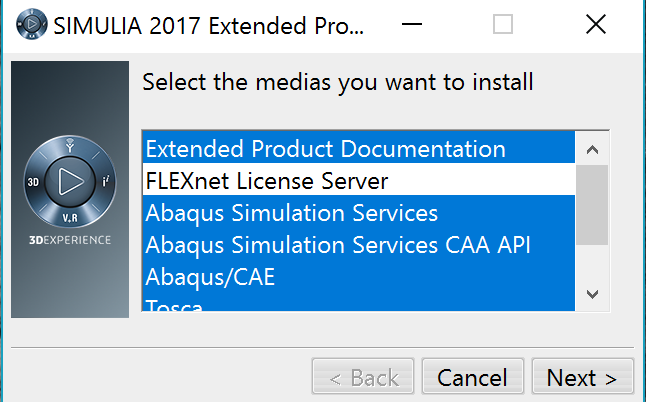
\includegraphics[width=8cm]{installer1.png} 
\caption{}
\label{fig:abaqus1}
\end{figure}
Please note you do not need installing the Flexnet license server as you will be using the University of Sheffield license server.

Separate individual installers will be launched for the different product, one after the other.

\subsection{Documentation (optional)}
The documentation installation is optional. Nonetheless it is highly recommended that you install the Abaqus documentation.

Once the installation has finished you can immediately access the documentation by opening:
 \path{C:\Program Files\Dassault Systemes\SIMULIA2017doc\DSSIMULIA_Established_homepage_English.html} in your web browser.

\subsection{Abaqus services (solvers)}
The following services are available:
\begin{itemize}
\item  Abaqus/Explicit Solver
\item Abaqus/Standard Solver
\item Cosimulation Services
\item ODB API Services
\end{itemize}
It is advisable that you install all the solvers unless you are absolutely sure you will not need one of the components. 


\subsection{Abaqus CAE}
Once the installer is running it will ask for you to select the type of license server for Abaqus. Choose FlexNet as the license type and enter the licenser server: \textbf{27000@abaquslm.shef.ac.uk} (Fig. \ref{fig:abaqus2})

\begin{figure}[ht]
\centering
	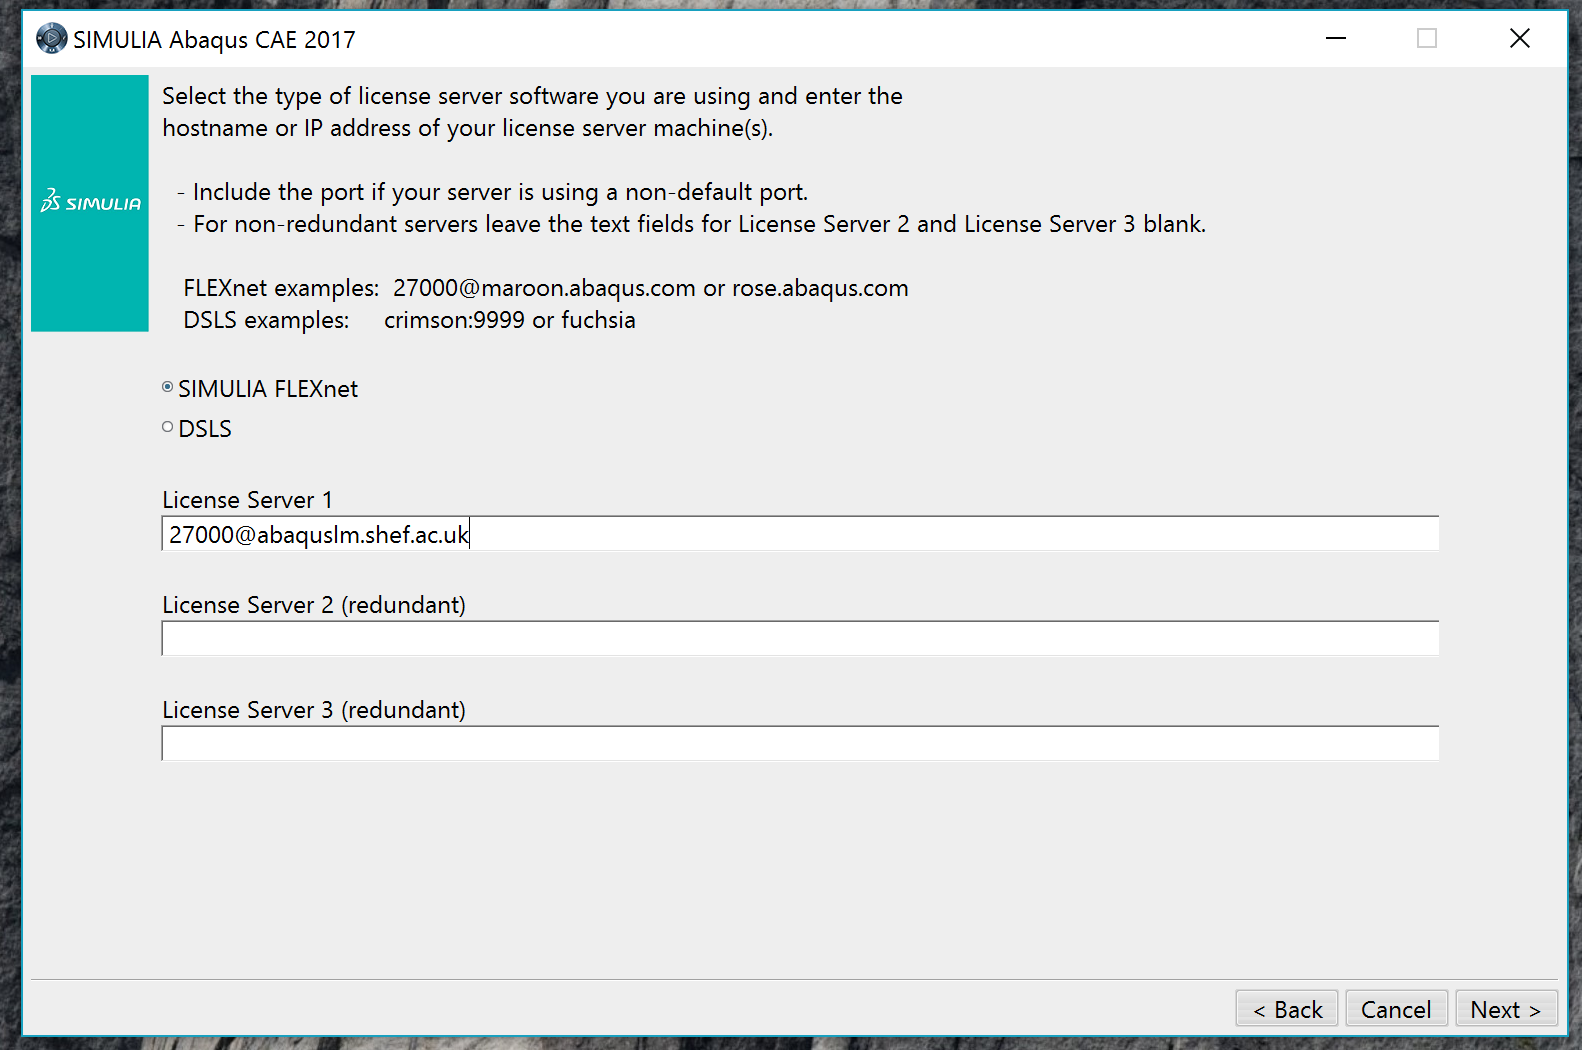
\includegraphics[width=14 cm, height=10 cm]{abaqus_license.png} 
	\caption{}
	\label{fig:abaqus2}
\end{figure}

When prompted to provide a location for the documentation select the path to your locally installed documentation. Alternatively, the URL for the served documentation can be found in \url{http://50.16.225.63} 

\textbf{Note}: the served documentation supports Abaqus versions 6.14, 2016 and 2017. If you want to directly point to the 2017 version documentation you need to go to \url{http://50.16.225.63} and log in directly to the 2917 version using your DS passport account (Fig. \ref{fig:abaqus3}).

\begin{figure}[ht]
\centering
	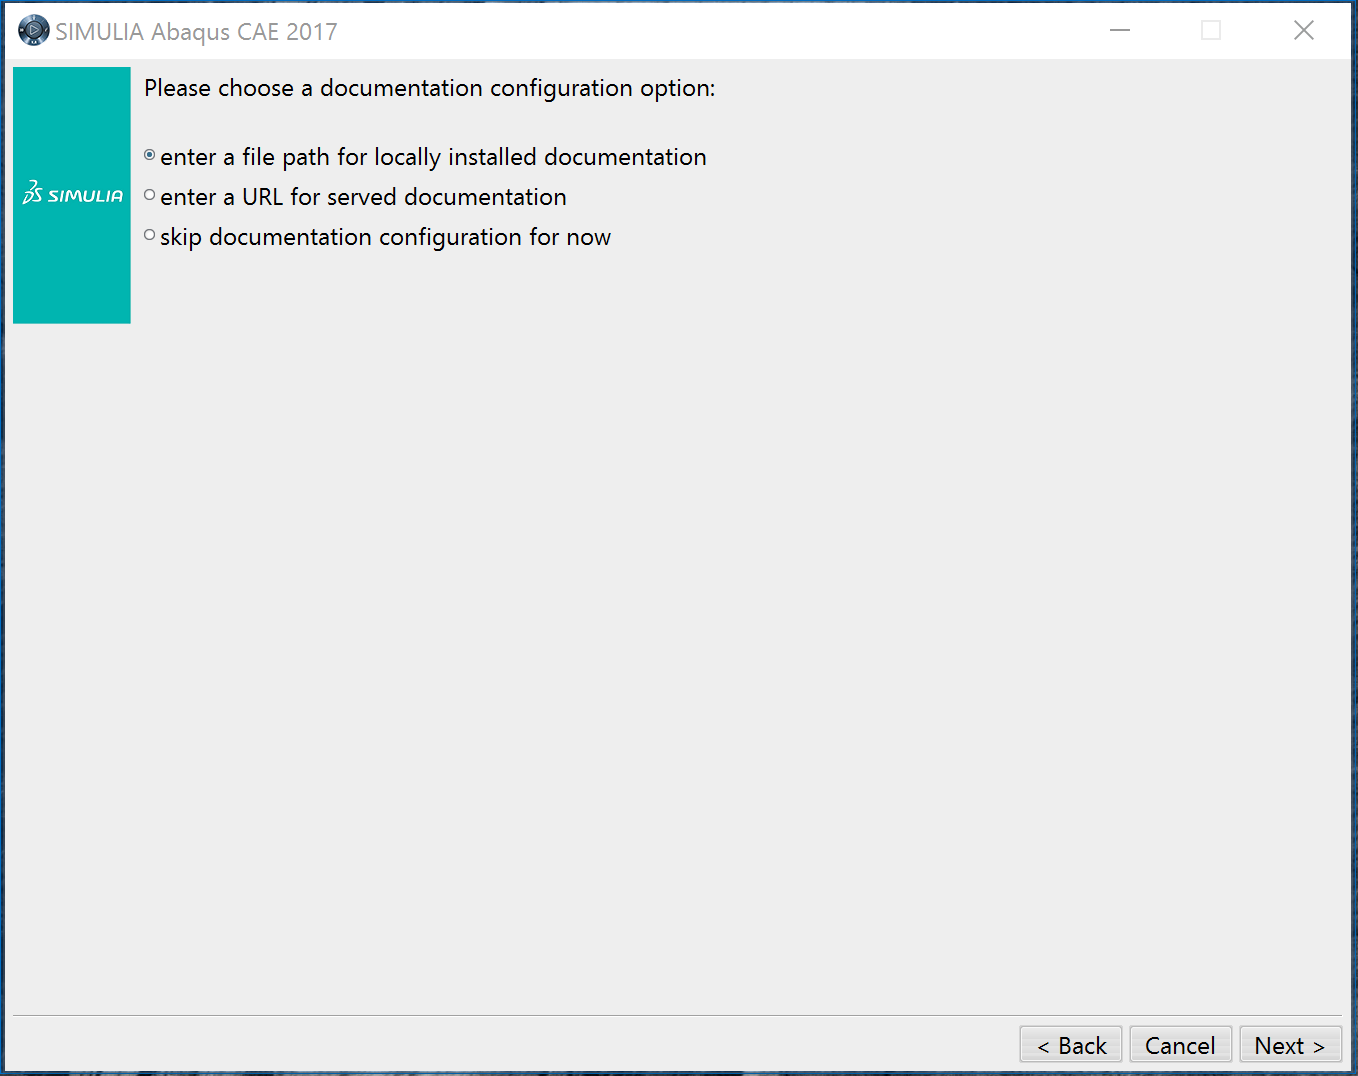
\includegraphics[width=14cm, height=10cm]{documentation_CAE.png} 
	\caption{}
	\label{fig:abaqus3}
\end{figure}


You will be asked to choose the location of you default working directory. By default this is \textbf{\path{C:\temp}} which will be created if it does not exist. If you want to choose a different location you must ensure this directory  exists. 

\section{Verification suite}
After Abaqus CAE has been installed a verification suite will be run and the results will be displayed. This is only a sub-set of the verification suite, so it is advisable that the verification is run after installation again. 

If you need to work with subroutines you need to complete the Post-Installation tasks detailed below before running the verification again.


\end{enumerate}

\section{Additional information}
If you select the default command locations the different products can be located in:
\begin{itemize}
\item The Abaqus launch command is abaqus (or abaqus cae for the GUI, abaqus viewer for the viewer) in the /var/DassaultSystemes/SIMULIA/Commands directory.
\item The fe-safe launch command is fe-safe, in the \path{/usr/SIMULIA/fe-safe/2017} directory.
\item The Isight launch command is gateway, in the \path{/usr/SIMULIA/Isight/2017/linux_a64/code/command } directory.
\item The Tosca Structure launch command is ToscaStructureGui.sh, in the \path{/usr/SIMULIA/Tosca/2017/linux_a64/code/command} directory.
\item The Tosca Fluid launch command is ToscaFluidGui.sh, in the \path{/usr/SIMULIA/Tosca/2017/linux_a64/code/command} directory.
\end{itemize}
\end{document}

 

